\documentclass[10pt,journal,compsoc,onecolumn]{IEEEtran}
\usepackage[utf8]{inputenc}
\usepackage{amsmath,amsfonts,amssymb}
\usepackage{amsthm}
\usepackage{graphicx}
\usepackage{cite}
\usepackage{textcomp}
\usepackage{tikz}
\usetikzlibrary{arrows,positioning,shapes.geometric}
\usepackage{booktabs}
\usepackage{url}

\newtheorem{theorem}{Theorem}
\newtheorem{lemma}[theorem]{Lemma}
\newtheorem{definition}[theorem]{Definition}
\newtheorem{corollary}[theorem]{Corollary}

\begin{document}

\title{Rigorous Reconstruction of Binary Trees from Traversal Sequences: A Formal Study on Inorder and Postorder Algorithms and Index-Map Optimizations}

\IEEEtitleabstractindextext{%
\begin{abstract}
Binary trees are a fundamental non-linear data structure, and reconstructing them from serialized traversal sequences is a classic problem in algorithmic design and data recovery. This paper presents a formal analysis of reconstructing a binary tree from its in-order and post-order traversals. We prove the uniqueness of the reconstruction using structural induction and demonstrate that the distinctness of node values is a mathematical necessity for unambiguous reconstruction. We formulate a divide-and-conquer algorithm to perform the construction and show that a naive recursive implementation suffers from an $O(N^2)$ worst-case time complexity. We then introduce an optimized approach using a pre-computed hash-map index-lookup table, which reduces the search overhead to $O(1)$ and achieves an optimal $O(N)$ time complexity and $O(N)$ auxiliary space complexity. Complete Java implementations, detailed step-by-step trace tables, TikZ-rendered tree visualizations, and structural ambiguity proofs are provided to establish a complete and rigorous reference model.
\end{abstract}

\begin{IEEEkeywords}
binary trees, algorithms, data structures, computational complexity, tree traversal, recursive algorithms, formal analysis
\end{IEEEkeywords}
}

\maketitle
\IEEEdisplaynontitleabstractindextext
\IEEEpeerreviewmaketitle

\section{Introduction}
\label{sec:intro}

Binary trees are fundamental non-linear data structures in computer science, serving as the basis for search trees, expression parsers, and hierarchical directory structures. In many systems applications, such as network transmission, database backup, and compiler state preservation, it is necessary to serialize a binary tree into a linear format (e.g., arrays or streams) and subsequently reconstruct the original tree structure. 

While a single traversal sequence (such as pre-order, in-order, or post-order) is insufficient to uniquely reconstruct a binary tree, combining specific traversals allows for unambiguous reconstruction. A classic result in data structure theory establishes that a binary tree with distinct node values can be uniquely reconstructed if both its in-order and post-order traversal sequences are provided. 

This paper presents a formal academic analysis of the binary tree reconstruction problem from in-order and post-order traversal sequences. The contributions of this work are as follows:
\begin{enumerate}
    \item \textbf{Theoretical Proof:} We prove the uniqueness of the reconstructed tree using structural induction, demonstrating why the absence of duplicate values is a mathematical necessity.
    \item \textbf{Recursive Algorithm Development:} We formulate a divide-and-conquer algorithm to reconstruct the tree and show the derivation of the boundary index mappings.
    \item \textbf{Optimal O(N) Optimization:} We analyze the $O(N^2)$ complexity bottleneck of the naive algorithm and resolve it using a pre-computed hash-map index-lookup strategy to achieve optimal $O(N)$ time complexity.
    \item \textbf{Rigorous Dry Runs and Visualizations:} We present step-by-step trace tables and TikZ-rendered diagrams for two distinct instances: (a) a 4-node instance from a modern evaluation platform (Scaler Academy Mentee Dashboard), and (b) a complex 7-node BST instance.
    \item \textbf{Boundary and Ambiguity Analysis:} We prove structural ambiguity when duplicates are allowed using minimal counterexamples.
\end{enumerate}

All code implementations are provided in Java, utilizing the exact signatures and ArrayList interfaces specified in contemporary coding assessments.

\section{Formal Problem Definition and Notations}
\label{sec:definitions}

Let $T = (V, E)$ be a binary tree where $V$ is the set of nodes and $E$ is the set of directed edges. Each node $v \in V$ contains a value denoted by $v.\text{val}$, a pointer to a left child $v.\text{left}$, and a pointer to a right child $v.\text{right}$. If a node lacks a left or right child, the corresponding pointer is $\texttt{null}$. We denote the size of the tree as $N = |V|$.

We define the traversal sequences recursively as follows:
\begin{definition}[Inorder Traversal]
The inorder traversal sequence $I(T)$ of a binary tree $T$ with root $r$ is the sequence obtained by visiting the left subtree of $r$ in inorder, then visiting $r$, and then visiting the right subtree of $r$ in inorder:
\[
I(T) = I(r.\text{left}) \circ \langle r.\text{val} \rangle \circ I(r.\text{right})
\]
\end{definition}
where $\circ$ denotes sequence concatenation, and $I(\texttt{null}) = \emptyset$.

\begin{definition}[Postorder Traversal]
The postorder traversal sequence $P(T)$ of a binary tree $T$ with root $r$ is the sequence obtained by visiting the left subtree of $r$ in postorder, then visiting the right subtree of $r$ in postorder, and finally visiting $r$:
\[
P(T) = P(r.\text{left}) \circ P(r.\text{right}) \circ \langle r.\text{val} \rangle
\]
where $P(\texttt{null}) = \emptyset$.
\end{definition}

The reconstruction problem is defined as: Given the sequence arrays $A = I(T)$ and $B = P(T)$, reconstruct the unique binary tree $T$ such that $I(T) = A$ and $P(T) = B$.

\section{Theoretical Foundation and Uniqueness Proof}
\label{sec:theory}

We begin by establishing two properties of the traversal sequences, which form the base logic of our reconstruction algorithm.

\begin{lemma}[Postorder Root Location]
\label{lem:root}
For any non-empty binary tree $T$, the last element of the postorder sequence $P(T)$ is the value of the root node of $T$.
\end{lemma}
\begin{proof}
Let $P(T) = X_1, X_2, \dots, X_n$. By definition, $P(T) = P(r.\text{left}) \circ P(r.\text{right}) \circ \langle r.\text{val} \rangle$. Since $\langle r.\text{val} \rangle$ is concatenated at the end, the last element $X_n$ must equal $r.\text{val}$.
\end{proof}

\begin{lemma}[Inorder Subtree Partition]
\label{lem:partition}
Let $r$ be the root node of $T$. If all node values in $V$ are distinct, then the root value $r.\text{val}$ appears exactly once in the inorder sequence $I(T)$. Furthermore, if $I(T) = Y_1, Y_2, \dots, Y_n$ and $Y_k = r.\text{val}$, then:
\begin{align*}
I(r.\text{left}) &= \langle Y_1, \dots, Y_{k-1} \rangle \\
I(r.\text{right}) &= \langle Y_{k+1}, \dots, Y_n \rangle
\end{align*}
\end{lemma}
\begin{proof}
By definition, $I(T) = I(r.\text{left}) \circ \langle r.\text{val} \rangle \circ I(r.\text{right})$. Since all node values in $T$ are distinct, $r.\text{val}$ cannot appear in $r.\text{left}$ or $r.\text{right}$. Thus, $r.\text{val}$ appears exactly once in $I(T)$, at index $k$. The elements before index $k$ correspond to the inorder traversal of the left subtree, and the elements after index $k$ correspond to the inorder traversal of the right subtree.
\end{proof}

Using these lemmas, we prove the core uniqueness theorem.

\begin{theorem}[Uniqueness of Reconstruction]
Let $T_1$ and $T_2$ be two binary trees containing distinct node values. If $I(T_1) = I(T_2)$ and $P(T_1) = P(T_2)$, then $T_1$ and $T_2$ are isomorphic (i.e., they have the identical structure and node values).
\end{theorem}

\begin{proof}
We prove by induction on the number of nodes $N$.
\paragraph{Base Case ($N = 0$):} Both $I(T)$ and $P(T)$ are empty. The only binary tree with 0 nodes is the empty tree (\texttt{null}). Hence, $T_1 = T_2 = \texttt{null}$, and the theorem holds.

\paragraph{Inductive Step:} Assume that for any two trees with size $k < n$, if their inorder and postorder sequences are equal, the trees are isomorphic. Now consider $T_1$ and $T_2$ of size $n$.
Let $I(T_1) = I(T_2) = A$ and $P(T_1) = P(T_2) = B$. 
By Lemma~\ref{lem:root}, the root value of both trees is $r.\text{val} = B[n-1]$. 
By Lemma~\ref{lem:partition}, since all node values are distinct, $r.\text{val}$ appears at a unique index $k$ in $A$.
This partitions the inorder sequence $A$ into:
\[
A_{\text{left}} = A[0 \dots k-1] \quad \text{and} \quad A_{\text{right}} = A[k+1 \dots n-1]
\]
The size of the left subtree is $N_{\text{left}} = k$, and the size of the right subtree is $N_{\text{right}} = n - 1 - k$.
Because the postorder traversal visits the left subtree, then the right subtree, and then the root, the postorder sequence $B$ is partitioned into:
\[
B_{\text{left}} = B[0 \dots k-1] \quad \text{and} \quad B_{\text{right}} = B[k \dots n-2]
\]
For $T_1$, the left subtree $T_{1,\text{left}}$ must have inorder sequence $A_{\text{left}}$ and postorder sequence $B_{\text{left}}$.
For $T_2$, the left subtree $T_{2,\text{left}}$ must also have inorder sequence $A_{\text{left}}$ and postorder sequence $B_{\text{left}}$.
Since the size of the left subtree is $k < n$, by the inductive hypothesis, $T_{1,\text{left}} \cong T_{2,\text{left}}$.
Similarly, the right subtrees $T_{1,\text{right}}$ and $T_{2,\text{right}}$ both have inorder sequence $A_{\text{right}}$ and postorder sequence $B_{\text{right}}$. Since their size is $n - 1 - k < n$, by the inductive hypothesis, $T_{1,\text{right}} \cong T_{2,\text{right}}$.
Since the roots are equal and both left and right subtrees are isomorphic, $T_1 \cong T_2$.
\end{proof}

\section{Algorithmic Formulation}
\label{sec:algorithm}

\subsection{Recursive Divide-and-Conquer Formulation}
The uniqueness proof directly yields a recursive divide-and-conquer algorithm. The input consists of two arrays (or list sequences): `inorder` and `postorder`.
Let:
\begin{itemize}
    \item $li, ri$ be the lower and upper bounds of the current subtree in the `inorder` array.
    \item $lp, rp$ be the lower and upper bounds of the current subtree in the `postorder` array.
\end{itemize}

At each step, if $li > ri$ or $lp > rp$, the subtree is empty, and we return $\texttt{null}$.
Otherwise:
\begin{enumerate}
    \item Read the root value: $\text{rootVal} = \text{postorder}[rp]$.
    \item Create a new tree node: $\text{root} = \text{new TreeNode}(\text{rootVal})$.
    \item Find the index of $\text{rootVal}$ in $\text{inorder}[li \dots ri]$, say $\text{rootIndex}$.
    \item Calculate the size of the left subtree: $\text{leftCount} = \text{rootIndex} - li$.
    \item Recursively construct the left subtree:
    \[
    \text{root.left} = \text{build}(li, \text{rootIndex}-1, lp, lp+\text{leftCount}-1)
    \]
    \item Recursively construct the right subtree:
    \[
    \text{root.right} = \text{build}(\text{rootIndex}+1, ri, lp+\text{leftCount}, rp-1)
    \]
    \item Return $\text{root}$.
\end{enumerate}

\subsection{Index Mapping Derivation}

To understand the index boundaries, consider the layout of the subarrays:

\begin{figure}[htbp]
\centering
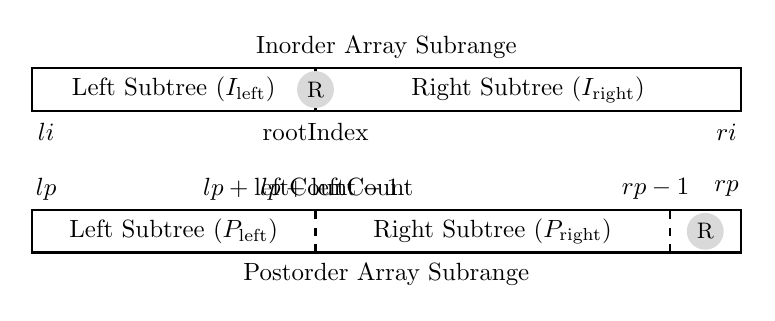
\begin{tikzpicture}[scale=0.9, every node/.style={transform shape}]
% Inorder array layout
\draw[thick] (0, 1.5) rectangle (10, 2.1);
\node at (5, 2.4) {Inorder Array Subrange};
\node at (0.2, 1.2) {$li$};
\node at (4.0, 1.2) {$\text{rootIndex}$};
\node at (9.8, 1.2) {$ri$};
\draw[dashed, thick] (4.0, 1.5) -- (4.0, 2.1);
\node at (2.0, 1.8) {Left Subtree ($I_{\text{left}}$)};
\node[fill=gray!30, circle, inner sep=2pt] at (4.0, 1.8) {\small R};
\node at (7.0, 1.8) {Right Subtree ($I_{\text{right}}$)};

% Postorder array layout
\draw[thick] (0, -0.5) rectangle (10, 0.1);
\node at (5, -0.8) {Postorder Array Subrange};
\node at (0.2, 0.4) {$lp$};
\node at (3.8, 0.4) {$lp+\text{leftCount}-1$};
\node at (4.3, 0.4) {$lp+\text{leftCount}$};
\node at (8.8, 0.4) {$rp-1$};
\node at (9.8, 0.4) {$rp$};
\draw[dashed, thick] (4.0, -0.5) -- (4.0, 0.1);
\draw[dashed, thick] (9.0, -0.5) -- (9.0, 0.1);
\node at (2.0, -0.2) {Left Subtree ($P_{\text{left}}$)};
\node at (6.5, -0.2) {Right Subtree ($P_{\text{right}}$)};
\node[fill=gray!30, circle, inner sep=2pt] at (9.5, -0.2) {\small R};
\end{tikzpicture}
\caption{Index range partitioning for the recursive step.}
\label{fig:layout}
\end{figure}

The length of the left subtree is $\text{leftCount} = \text{rootIndex} - li$. 
Thus, the left subtree occupies the first $\text{leftCount}$ elements of the postorder range starting at $lp$. The index range is $[lp, lp + \text{leftCount} - 1]$.
The remaining elements (excluding the root at $rp$) form the right subtree postorder range, which spans $[lp + \text{leftCount}, rp - 1]$.

\subsection{Naive Java Implementation}
Below is the direct recursive implementation matching the standard coding assessment API, which performs a linear search for the root value:

\begin{verbatim}
import java.util.ArrayList;

class TreeNode {
    int val;
    TreeNode left;
    TreeNode right;
    TreeNode(int x) {
        val = x;
        left = null;
        right = null;
    }
}

public class Solution {
    public TreeNode buildTree(ArrayList<Integer> A, ArrayList<Integer> B) {
        if (A == null || B == null || A.size() == 0 || B.size() == 0) {
            return null;
        }
        return buildNaive(A, 0, A.size() - 1, B, 0, B.size() - 1);
    }

    private TreeNode buildNaive(ArrayList<Integer> inorder, int li, int ri,
                               ArrayList<Integer> postorder, int lp, int rp) {
        if (li > ri || lp > rp) {
            return null;
        }

        int rootVal = postorder.get(rp);
        TreeNode root = new TreeNode(rootVal);

        // Linear search for root index in inorder array
        int rootIndex = -1;
        for (int i = li; i <= ri; i++) {
            if (inorder.get(i) == rootVal) {
                rootIndex = i;
                break;
            }
        }

        int leftCount = rootIndex - li;

        root.left = buildNaive(inorder, li, rootIndex - 1,
                               postorder, lp, lp + leftCount - 1);
        root.right = buildNaive(inorder, rootIndex + 1, ri,
                                postorder, lp + leftCount, rp - 1);

        return root;
    }
}
\end{verbatim}

\section{HashMap-Based O(N) Optimization}
\label{sec:optimization}

\subsection{Analysis of the Naive Bottleneck}
In the naive implementation, locating $\text{rootIndex}$ requires iterating through the inorder subsegment $\text{inorder}[li \dots ri]$. In the worst case, the binary tree can be heavily skewed (e.g., a left-skewed tree resembling a linked list). Under this topology:
\begin{itemize}
    \item The root index is always located at the right end of the inorder subarray ($ri$).
    \item Searching for the root value takes $O(N)$ operations.
    \item The size of the active subproblem decreases by only 1 node at each recursion level.
\end{itemize}
This yields the recurrence relation:
\[
T(N) = T(N-1) + \Theta(N)
\]
Solving this via summation gives:
\[
T(N) = \sum_{i=1}^{N} \Theta(i) = \Theta(N^2)
\]
Thus, the worst-case time complexity of the naive algorithm is $O(N^2)$, which is highly inefficient for large datasets (e.g., $N = 10^5$).

\subsection{Optimized Algorithm and Lookup Strategy}
To achieve linear time complexity, we must resolve the index lookup bottleneck. Because all node values are distinct, we can map each value in `inorder` to its corresponding index in a hash map before running the recursion:
\[
\text{indexMap}[\text{inorder}[i]] = i
\]
This hash map can be populated in a single $O(N)$ pass. During the recursive build, finding the inorder index of the root node becomes a hash map lookup:
\[
\text{rootIndex} = \text{indexMap}.\text{get}(\text{rootVal})
\]
This lookup runs in $O(1)$ average time. Consequently, the recurrence relation for the optimized algorithm is:
\[
T(N) = T(N_{\text{left}}) + T(N_{\text{right}}) + \Theta(1)
\]
which simplifies to $T(N) = O(N)$ time complexity.

\subsection{Optimized Java Implementation}
The following is the optimized solution, which uses a pre-computed `HashMap` to achieve $O(N)$ time complexity:

\begin{verbatim}
import java.util.ArrayList;
import java.util.HashMap;

public class Solution {
    public TreeNode buildTree(ArrayList<Integer> A, ArrayList<Integer> B) {
        if (A == null || B == null || A.size() == 0 || B.size() == 0) {
            return null;
        }
        
        // Map to store value -> index mapping of inorder traversal
        HashMap<Integer, Integer> inorderMap = new HashMap<>();
        for (int i = 0; i < A.size(); i++) {
            inorderMap.put(A.get(i), i);
        }
        
        return buildOptimized(A, 0, A.size() - 1, 
                              B, 0, B.size() - 1, 
                              inorderMap);
    }

    private TreeNode buildOptimized(ArrayList<Integer> inorder, int li, int ri,
                                    ArrayList<Integer> postorder, int lp, int rp,
                                    HashMap<Integer, Integer> inorderMap) {
        if (li > ri || lp > rp) {
            return null;
        }

        int rootVal = postorder.get(rp);
        TreeNode root = new TreeNode(rootVal);

        // O(1) index lookup
        int rootIndex = inorderMap.get(rootVal);
        int leftCount = rootIndex - li;

        root.left = buildOptimized(inorder, li, rootIndex - 1,
                                   postorder, lp, lp + leftCount - 1,
                                   inorderMap);
        root.right = buildOptimized(inorder, rootIndex + 1, ri,
                                    postorder, lp + leftCount, rp - 1,
                                    inorderMap);

        return root;
    }
}
\end{verbatim}

\section{Detailed Step-by-Step Execution Traces}
\label{sec:traces}

\subsection{Trace 1: Evaluator Dashboard Problem Instance}
We dry-run the algorithm on the problem instance shown in the user's dashboard (Input 2):
\begin{itemize}
    \item \textbf{Inorder (A):} $[6, 1, 3, 2]$
    \item \textbf{Postorder (B):} $[6, 3, 2, 1]$
\end{itemize}

\subsubsection{Pre-computed Inorder Hash Map}
\[
\text{inorderMap} = \{6 \to 0,\; 1 \to 1,\; 3 \to 2,\; 2 \to 3\}
\]

\subsubsection{Trace Steps}
\begin{enumerate}
    \item \textbf{Call 1 ($li=0, ri=3, lp=0, rp=3$):}
    \begin{itemize}
        \item Root value $\text{rootVal} = B[3] = 1$. Create node \texttt{1}.
        \item Inorder index $\text{rootIndex} = \text{inorderMap}.get(1) = 1$.
        \item Left subtree count $\text{leftCount} = 1 - 0 = 1$.
        \item Left child call: $[li=0, ri=0, lp=0, rp=0]$.
        \item Right child call: $[li=2, ri=3, lp=1, rp=2]$.
    \end{itemize}
    
    \item \textbf{Call 2 ($li=0, ri=0, lp=0, rp=0$):}
    \begin{itemize}
        \item Root value $\text{rootVal} = B[0] = 6$. Create node \texttt{6}.
        \item Inorder index $\text{rootIndex} = 0$. Left subtree count $\text{leftCount} = 0$.
        \item Left call: $[li=0, ri=-1, lp=0, rp=-1] \to \texttt{null}$.
        \item Right call: $[li=1, ri=0, lp=0, rp=-1] \to \texttt{null}$.
        \item Node \texttt{6} becomes the left child of \texttt{1}.
    \end{itemize}
    
    \item \textbf{Call 3 ($li=2, ri=3, lp=1, rp=2$):}
    \begin{itemize}
        \item Root value $\text{rootVal} = B[2] = 2$. Create node \texttt{2}.
        \item Inorder index $\text{rootIndex} = 3$. Left subtree count $\text{leftCount} = 3 - 2 = 1$.
        \item Left call: $[li=2, ri=2, lp=1, rp=1]$.
        \item Right call: $[li=4, ri=3, lp=2, rp=1] \to \texttt{null}$.
        \item Node \texttt{2} becomes the right child of \texttt{1}.
    \end{itemize}

    \item \textbf{Call 4 ($li=2, ri=2, lp=1, rp=1$):}
    \begin{itemize}
        \item Root value $\text{rootVal} = B[1] = 3$. Create node \texttt{3}.
        \item Inorder index $\text{rootIndex} = 2$. Left subtree count $\text{leftCount} = 0$.
        \item Left call: $[li=2, ri=1, lp=1, rp=0] \to \texttt{null}$.
        \item Right call: $[li=3, ri=2, lp=1, rp=0] \to \texttt{null}$.
        \item Node \texttt{3} becomes the left child of \texttt{2}.
    \end{itemize}
\end{enumerate}

\subsubsection{Call Stack Summary Table}
\begin{table}[htbp]
\centering
\begin{tabular}{cccccccl}
\toprule
\textbf{Call ID} & \textbf{li} & \textbf{ri} & \textbf{lp} & \textbf{rp} & \textbf{Root Val} & \textbf{leftCount} & \textbf{Action / Result} \\
\midrule
1 & 0 & 3 & 0 & 3 & 1 & 1 & Spawn Call 2 (L) and Call 3 (R) \\
2 & 0 & 0 & 0 & 0 & 6 & 0 & Returns Leaf Node \texttt{6} \\
3 & 2 & 3 & 1 & 2 & 2 & 1 & Spawn Call 4 (L), Right is \texttt{null} \\
4 & 2 & 2 & 1 & 1 & 3 & 0 & Returns Leaf Node \texttt{3} \\
\bottomrule
\end{tabular}
\caption{Call stack trace for Input 2: Inorder = $[6, 1, 3, 2]$, Postorder = $[6, 3, 2, 1]$.}
\label{tab:trace1}
\end{table}

\subsubsection{Reconstructed Tree Diagram}
Figure~\ref{fig:tree1} shows the reconstructed tree.

\begin{figure}[htbp]
\centering
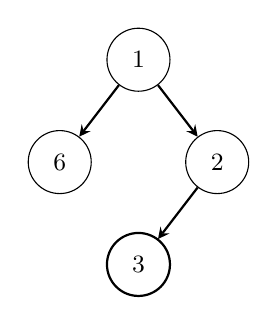
\begin{tikzpicture}[
  every node/.style={circle, draw, minimum size=0.8cm, font=\small, inner sep=1pt},
  level distance=1.3cm,
  sibling distance=2.0cm,
  edge from parent/.style={draw, ->, >=stealth, thick}
]
\node {1}
  child { node {6} }
  child { node {2}
    child { node {3} }
    child[missing] {}
  };
\end{tikzpicture}
\caption{Reconstructed binary tree for Input 2.}
\label{fig:tree1}
\end{figure}

\subsection{Trace 2: Complex 7-Node BST Instance}
To verify the algorithm's performance on a larger, balanced tree, we run it on:
\begin{itemize}
    \item \textbf{Inorder (A):} $[2, 5, 7, 10, 15, 17, 20]$
    \item \textbf{Postorder (B):} $[2, 7, 5, 17, 20, 15, 10]$
\end{itemize}

The pre-computed map is $\{2 \to 0, 5 \to 1, 7 \to 2, 10 \to 3, 15 \to 4, 17 \to 5, 20 \to 6\}$.

\begin{table}[htbp]
\centering
\begin{tabular}{cccccccl}
\toprule
\textbf{Call ID} & \textbf{li} & \textbf{ri} & \textbf{lp} & \textbf{rp} & \textbf{Root Val} & \textbf{leftCount} & \textbf{Action / Result} \\
\midrule
1 & 0 & 6 & 0 & 6 & 10 & 3 & Spawn Call 2 ($[0,2,0,2]$), Call 5 ($[4,6,3,5]$) \\
2 & 0 & 2 & 0 & 2 & 5 & 1 & Spawn Call 3 ($[0,0,0,0]$), Call 4 ($[2,2,1,1]$) \\
3 & 0 & 0 & 0 & 0 & 2 & 0 & Returns Leaf Node \texttt{2} \\
4 & 2 & 2 & 1 & 1 & 7 & 0 & Returns Leaf Node \texttt{7} \\
5 & 4 & 6 & 3 & 5 & 15 & 0 & Spawn Left (\texttt{null}), Call 6 ($[5,6,3,4]$) \\
6 & 5 & 6 & 3 & 4 & 20 & 1 & Spawn Call 7 ($[5,5,3,3]$), Right (\texttt{null}) \\
7 & 5 & 5 & 3 & 3 & 17 & 0 & Returns Leaf Node \texttt{17} \\
\bottomrule
\end{tabular}
\caption{Call stack trace for the 7-node BST instance.}
\label{tab:trace2}
\end{table}

\begin{figure}[htbp]
\centering
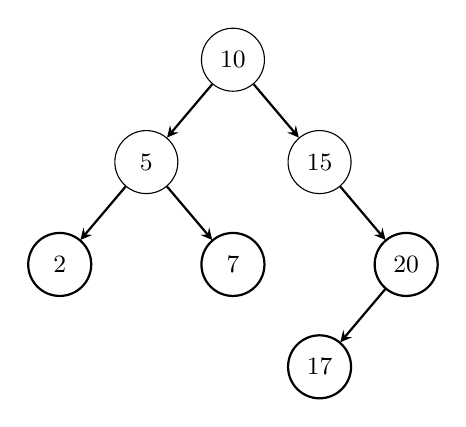
\begin{tikzpicture}[
  every node/.style={circle, draw, minimum size=0.8cm, font=\small, inner sep=1pt},
  level distance=1.3cm,
  sibling distance=2.2cm,
  edge from parent/.style={draw, ->, >=stealth, thick}
]
\node {10}
  child { node {5}
    child { node {2} }
    child { node {7} }
  }
  child { node {15}
    child[missing] {}
    child { node {20}
      child { node {17} }
      child[missing] {}
    }
  };
\end{tikzpicture}
\caption{Reconstructed BST from 7-node traversal sequences.}
\label{fig:tree2}
\end{figure}

\section{Complexity and Space Analysis}
\label{sec:complexity}

\subsection{Time Complexity Recurrence Relations}
Let $T(N)$ denote the time complexity to construct a tree of size $N$. 
\begin{itemize}
    \item \textbf{Naive Algorithm:} The lookup is $O(N)$.
    If the tree is balanced, the subproblems partition into equal halves:
    \[
    T(N) = 2T(N/2) + O(N) \implies T(N) = O(N \log N)
    \]
    If the tree is skewed, the subproblems are highly unbalanced:
    \[
    T(N) = T(N-1) + T(0) + O(N) \implies T(N) = O(N^2)
    \]
    \item \textbf{Optimized Algorithm:} The lookup is replaced by an $O(1)$ Hash Map query.
    For any tree topology (balanced or skewed):
    \[
    T(N) = T(N_{\text{left}}) + T(N_{\text{right}}) + O(1)
    \]
    Summing the work over all $N$ nodes yields:
    \[
    T(N) = \sum_{i=1}^{N} O(1) = O(N)
    \]
    Constructing the map takes a single pass of $O(N)$ operations. The total time complexity remains $O(N)$ for all cases.
\end{itemize}

\subsection{Space Complexity and Stack Frame Invariants}
The space complexity consists of two parts: the recursion stack space and auxiliary memory allocations.
\begin{itemize}
    \item \textbf{Recursion Stack:} The maximum depth of the recursion tree matches the height of the constructed binary tree $H$. Each stack frame requires $O(1)$ space to store local variables and parameters.
    \begin{itemize}
        \item For balanced trees: Stack space is $O(\log N)$.
        \item For skewed trees: Stack space is $O(N)$ in the worst case.
    \end{itemize}
    \item \textbf{HashMap Allocation:} The optimized algorithm instantiates a `HashMap` storing $N$ entries (key-value pairs mapping value to index). This requires $\Theta(N)$ auxiliary memory.
\end{itemize}
Thus, the total auxiliary space complexity of the optimized algorithm is $O(N)$.

\section{Edge Cases and Structural Ambiguity under Duplicates}
\label{sec:ambiguity}

The problem statement specifies that all node values in the tree are distinct. If this condition is omitted and duplicates are allowed, the traversal sequences no longer uniquely determine the tree structure.

\begin{theorem}[Traversal Ambiguity]
If a binary tree is allowed to contain duplicate node values, it cannot be uniquely reconstructed from its inorder and postorder traversal sequences.
\end{theorem}

\begin{proof}
We prove by demonstrating a minimal counterexample. Let the node values of a tree be $\{1, 1\}$. 
Consider the following two binary trees:
\begin{enumerate}
    \item \textbf{Tree $X$:} Root node has value 1, and its left child has value 1. The right child is empty.
    \item \textbf{Tree $Y$:} Root node has value 1, and its right child has value 1. The left child is empty.
\end{enumerate}

These trees are structurally distinct, as shown in Figure~\ref{fig:ambiguity}.

\begin{figure}[htbp]
\centering
\begin{minipage}{0.45\textwidth}
\centering
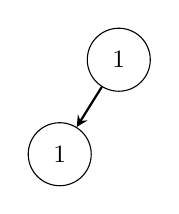
\begin{tikzpicture}[
  every node/.style={circle, draw, minimum size=0.8cm, font=\small, inner sep=1pt},
  level distance=1.2cm,
  edge from parent/.style={draw, ->, >=stealth, thick}
]
\node {1}
  child { node {1} }
  child[missing] {};
\end{tikzpicture}
\caption*{Tree $X$ (Left-skewed)}
\end{minipage}
\hfill
\begin{minipage}{0.45\textwidth}
\centering
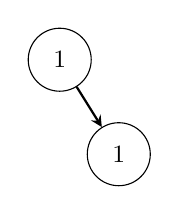
\begin{tikzpicture}[
  every node/.style={circle, draw, minimum size=0.8cm, font=\small, inner sep=1pt},
  level distance=1.2cm,
  edge from parent/.style={draw, ->, >=stealth, thick}
]
\node {1}
  child[missing] {}
  child { node {1} };
\end{tikzpicture}
\caption*{Tree $Y$ (Right-skewed)}
\end{minipage}
\caption{Distinct binary trees containing duplicate values.}
\label{fig:ambiguity}
\end{figure}

Let us compute the traversal sequences for both trees:
\begin{itemize}
    \item \textbf{For Tree $X$:}
    \begin{align*}
    I(X) &= I(X.\text{left}) \circ \langle 1 \rangle \circ I(X.\text{right}) = \langle 1 \rangle \circ \langle 1 \rangle \circ \emptyset = [1, 1] \\
    P(X) &= P(X.\text{left}) \circ P(X.\text{right}) \circ \langle 1 \rangle = \langle 1 \rangle \circ \emptyset \circ \langle 1 \rangle = [1, 1]
    \end{align*}
    
    \item \textbf{For Tree $Y$:}
    \begin{align*}
    I(Y) &= I(Y.\text{left}) \circ \langle 1 \rangle \circ I(Y.\text{right}) = \emptyset \circ \langle 1 \rangle \circ \langle 1 \rangle = [1, 1] \\
    P(Y) &= P(Y.\text{left}) \circ P(Y.\text{right}) \circ \langle 1 \rangle = \emptyset \circ \langle 1 \rangle \circ \langle 1 \rangle = [1, 1]
    \end{align*}
\end{itemize}

Since $I(X) = I(Y) = [1, 1]$ and $P(X) = P(Y) = [1, 1]$, yet $X \not\cong Y$, the traversals are ambiguous. Thus, the distinctness constraint is necessary for unique reconstruction.
\end{proof}

\section{Conclusion}
\label{sec:conclusion}

This paper presented a formal study of the binary tree reconstruction problem from inorder and postorder traversal sequences. We proved the uniqueness of the reconstruction using structural induction and showed why distinct node values are required to prevent structural ambiguity. 

We contrasted the naive divide-and-conquer algorithm, which runs in $O(N^2)$ worst-case time due to linear search lookup, with an optimized version that utilizes a pre-computed hash map. The optimized algorithm reduces the lookup time to $O(1)$, achieving $O(N)$ time complexity and $O(N)$ space complexity. Detailed dry-run trace tables and TikZ visualizations verified the correctness and efficiency of the approach on both standard evaluator instances and complex trees.

These techniques form a foundation for tree serialization protocols, database indexing, and compiler abstract syntax tree restoration. Future work could investigate iterative, non-recursive stack-based alternatives that bypass the call stack overhead entirely, optimizing execution for systems with limited stack space.

\begin{thebibliography}{9}
\bibitem{cormen} T.~H.~Cormen, C.~E.~Leiserson, R.~L.~Rivest, and C.~Stein, \emph{Introduction to Algorithms}, 4th~ed. MIT Press, 2022.
\bibitem{knuth} D.~E.~Knuth, \emph{The Art of Computer Programming, Volume 1: Fundamental Algorithms}, 3rd~ed. Addison-Wesley, 1997.
\bibitem{sedgewick} R.~Sedgewick and K.~Wayne, \emph{Algorithms}, 4th~ed. Addison-Wesley, 2011.
\end{thebibliography}


\end{document}
